\documentclass {article}
\usepackage{graphicx} % Required for inserting images
\usepackage{hyperref} % To make url look clean
\usepackage{url} % this is to make sure of the format
\begin{figure}
    \centering
    
\includegraphics[width=0.95\linewidth]{Screenshot 2026-06-26 at 16.30.00.png}
    \caption{}
    \label{fig:placeholder}
\end{figure}
\title{Computer Science Lab}
\author{Ayusha Subedi \\ GH Number: GH 1047076}
\date{24 June 2026}

\begin{document}

\maketitle
\newpage

\section{Introduction}
This report consists of my content for portfolio website and how I made it. I dive in to this project to showcase who I am and what are my skills and qualities are.This project will be an aid for me to initiate my carrer. Through this platform I am able to share all of my coding projects, the courses I've taken,and access of my social id.I will also explain how I made my CV using a Latex file,and talk about the decisions I made during the personal projects and describe the tools and technologies I used.To concise it, I will reflect on things that went well,the gaps I have and the procedure I will take to enhance my portfolio in future.
\subsection{
The links for my portfolio website, github and C.V can be accessed through the following links :}
\begin{itemize}
    \item \textbf{Portfolio Website:} \\  \url{https://ayushasubedi23.github.io/Portfolio-computer-lab-/ }
    \item \textbf{Github Repository} \\ \url{https://github.com/AyushaSubedi23?tab=repositories}
    \item \textbf{C.V} \\ \url{https://github.com/AyushaSubedi23/C.V}
\end{itemize}
\section{ Portfolio Overview \& Core Objectives }
The main objective of this portfolio is to develop an impactful digital presence.It showcases my skills and the projects I have done.As a Software Engineering student making this portfolio by applying real practical methodologies of theoretical knowledge feels like a critical milestone.This project is a live evidence of my ability to build a responsive interferance,create and manage repositories and present information with visual clarity.
The portfolio is based on four primary goals 
\begin{itemize}
    \item \textbf{Identity verification:} Starting my background as a Software Engineering student with advanced professional skills.
\item \textbf{Technical Validation} Providing with credible evidence of technical skills through showcasing live demonstration and source code of foundational applications (eg: Python scripts and interactive responsive designs.
\item \textbf{Resource Accessibility:}Allowing recruiters to easily download my latex CV and go through the code history on Github with a single touch 
\end{itemize}
\newpage
\section{Portfolio Website structure}
This website follows a very primitive single-page portfolio design.Responsive features were added using CSS Flexbox and media queries to ensure compatibility to view in different screens.

\subsection{Home Page}
The home page introduce a bit of me and the portfolio itself.
\begin{figure}[h]
    \centering
    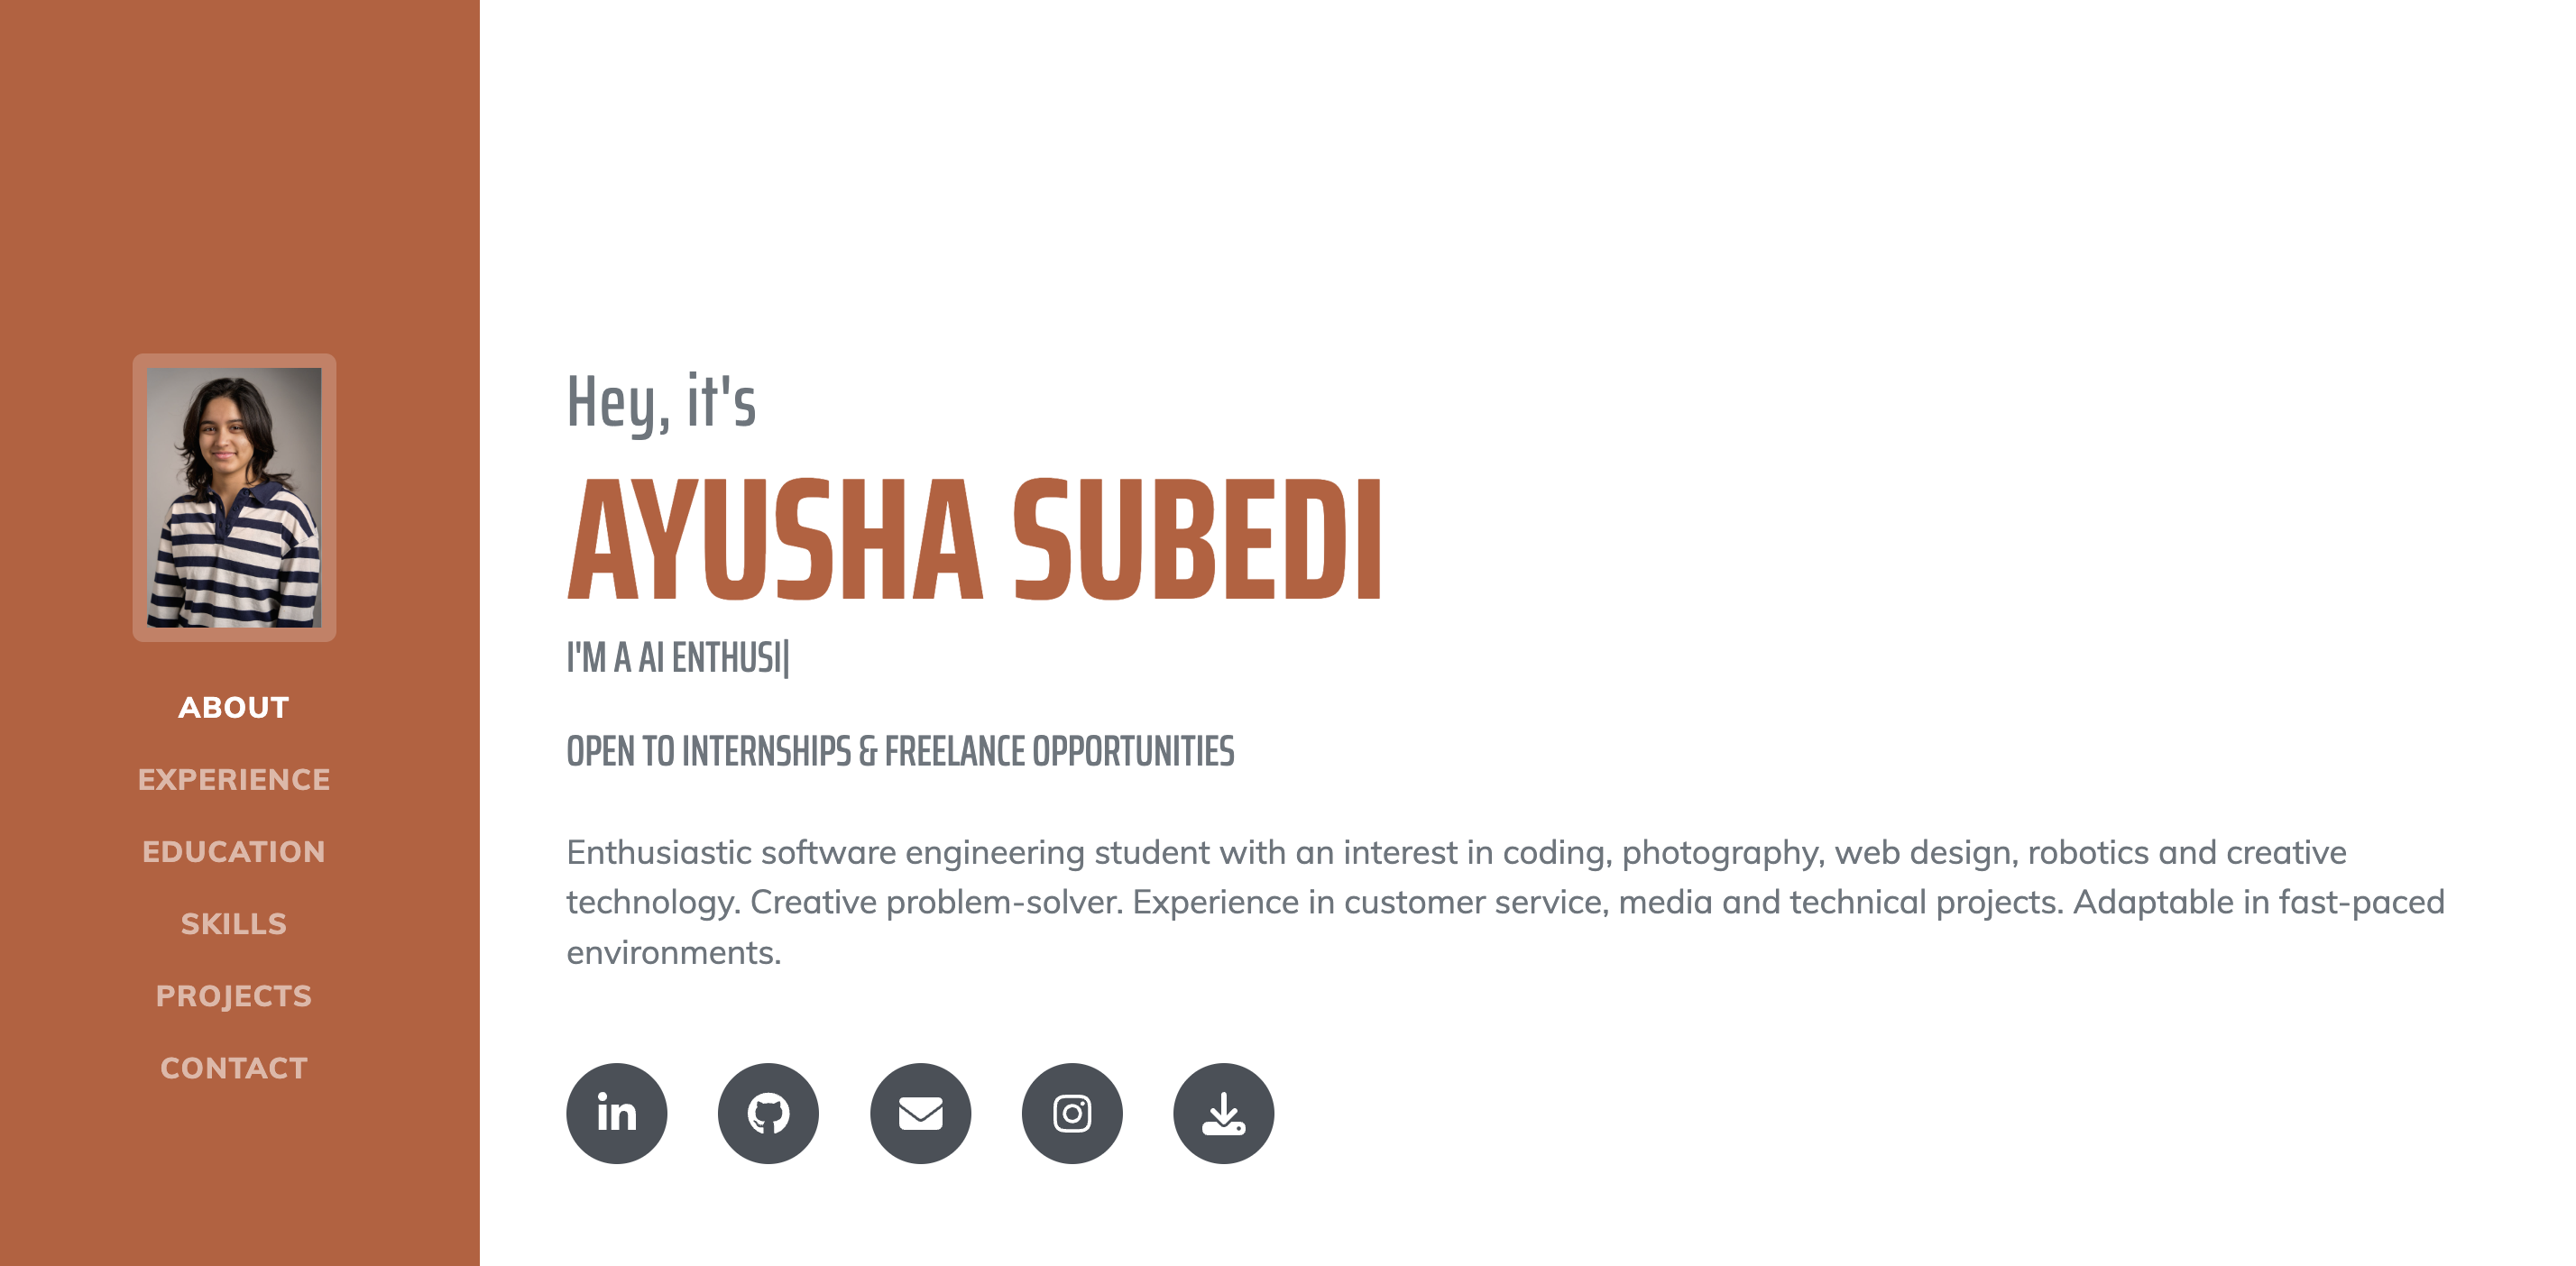
\includegraphics[width=0.75\linewidth]{Screenshot 2026-06-26 at 14.51.10.png}
    \caption{Home page}
    \label{fig:home_page}
\end{figure}
\subsection{Work experience}
In this section I showcase all of the work experiences I had with a bit of ahat I gain experience from.

\begin{figure}[h]
        \centering
        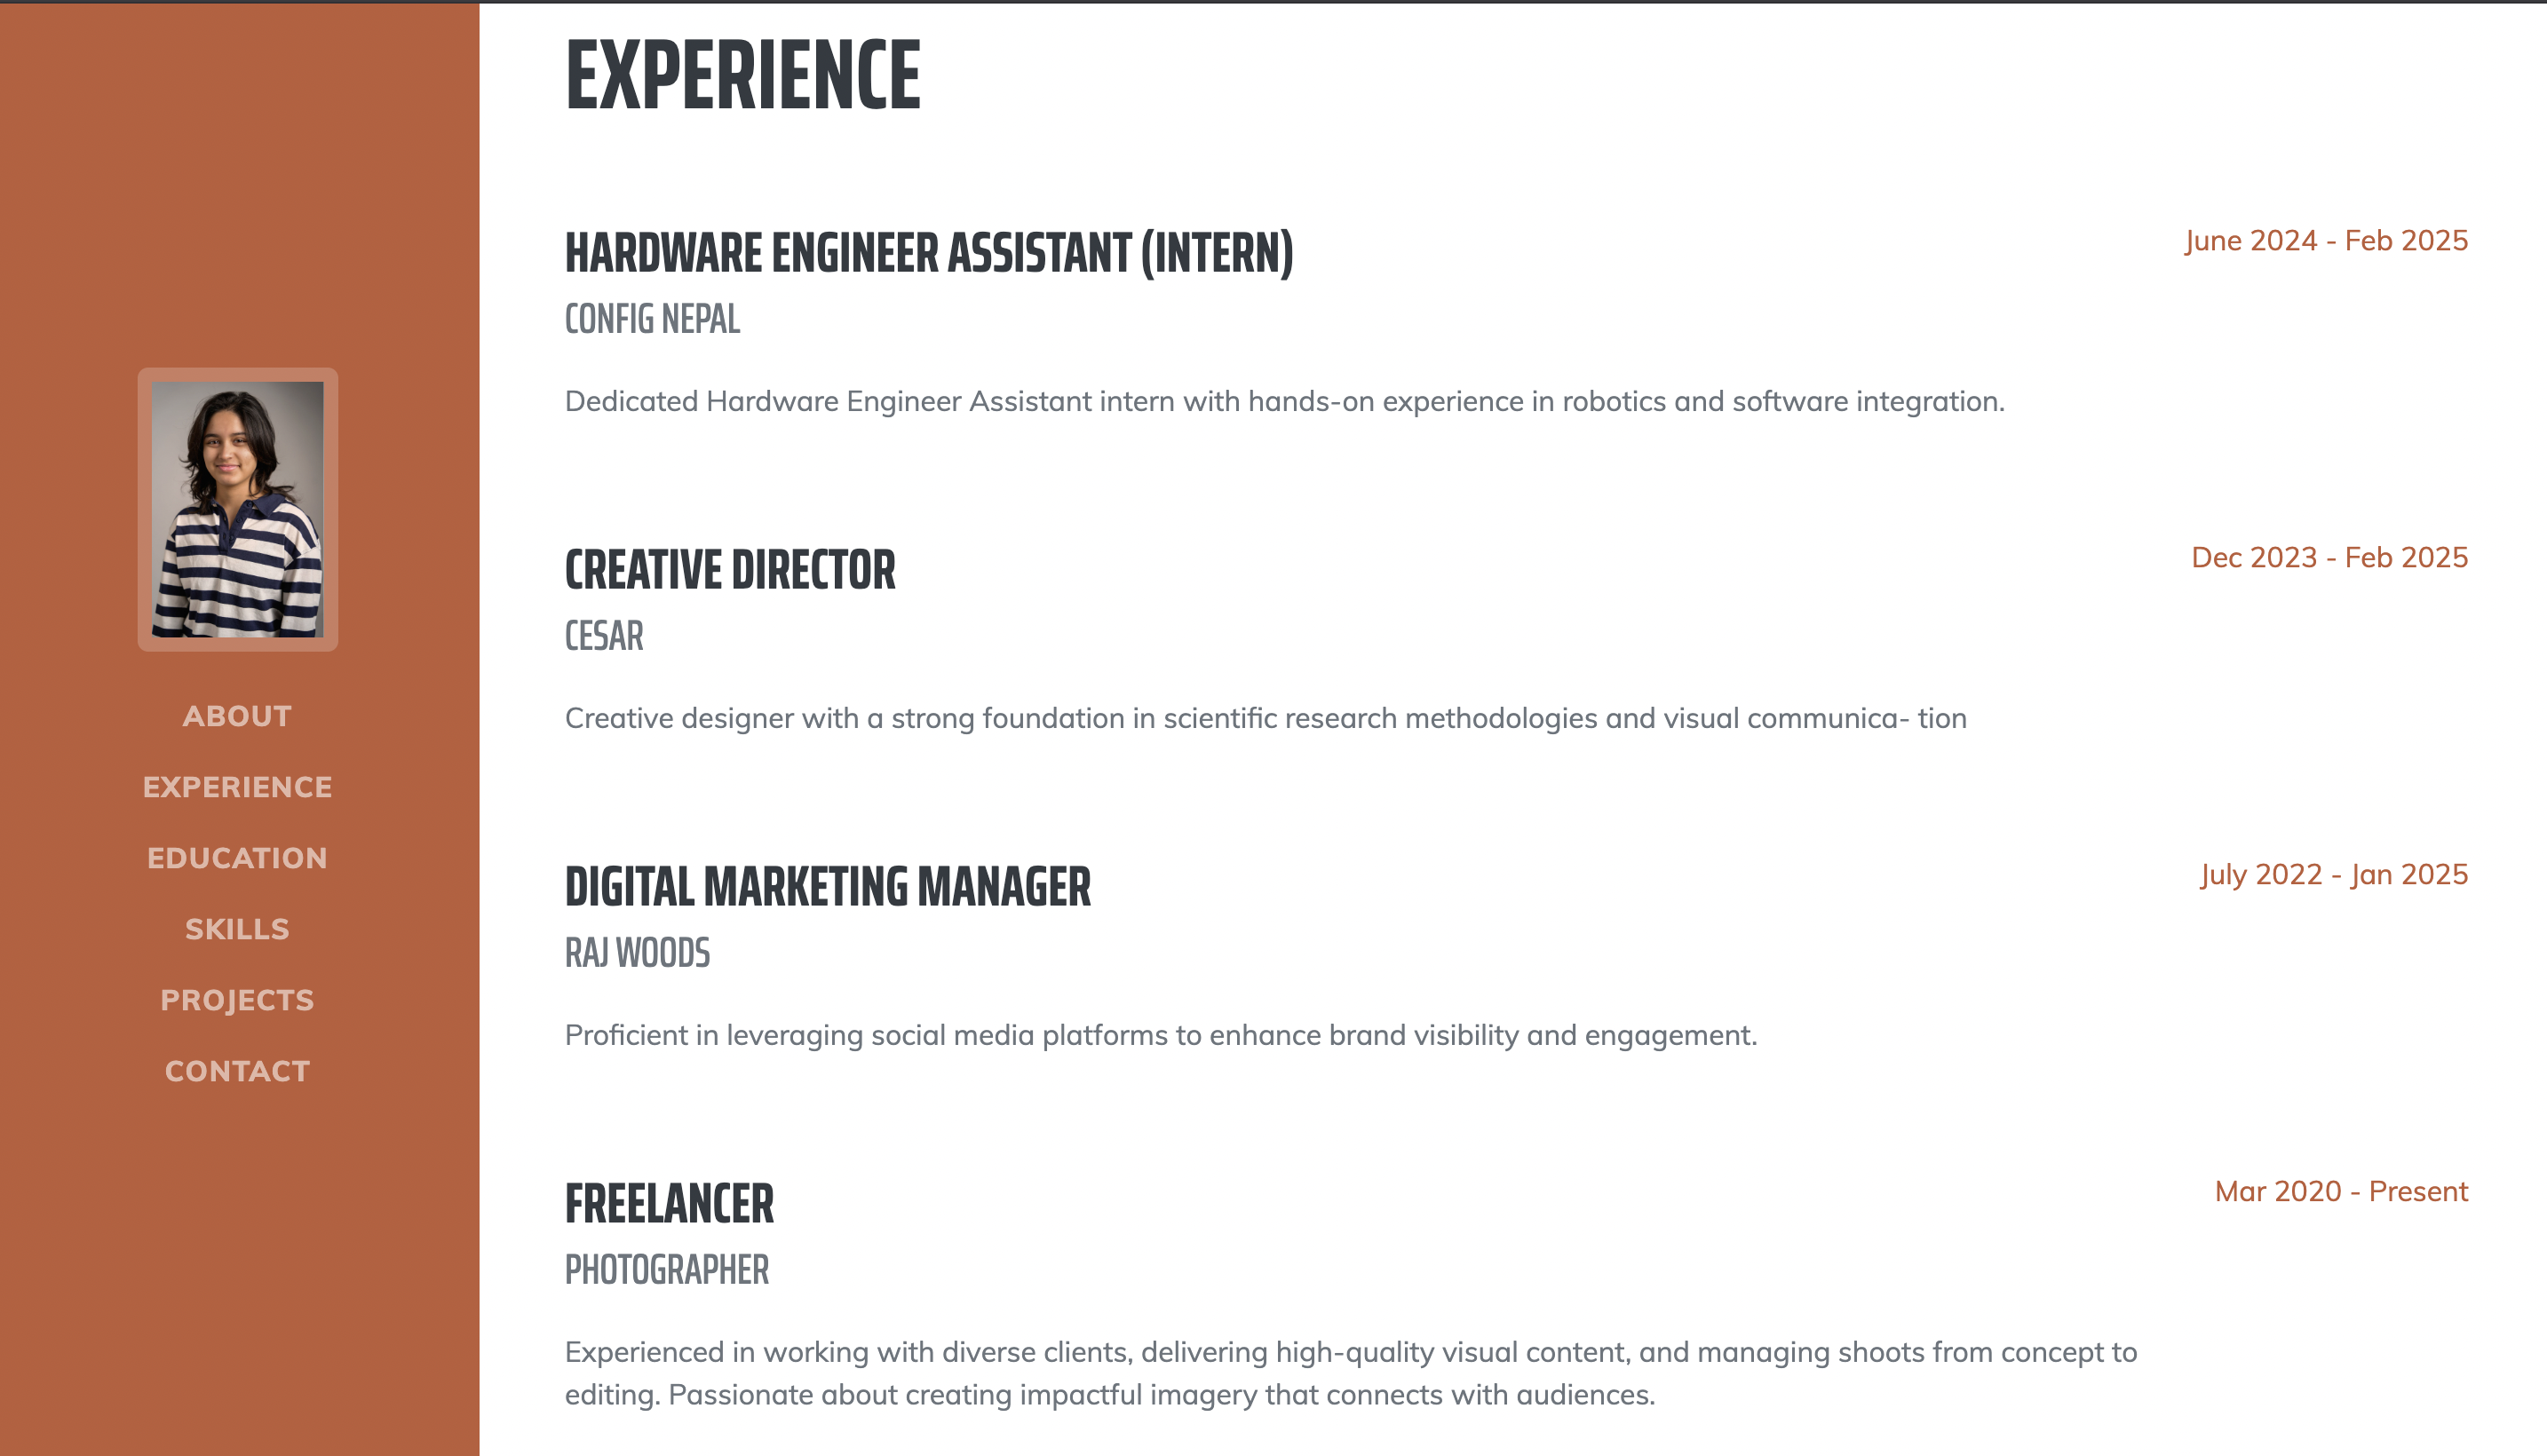
\includegraphics[width=0.75\linewidth]{Screenshot 2026-06-26 at 15.04.45.png}
        \caption{work experience}
        \label{fig:work_experience}
    \end{figure}
\subsection{Education}
In this section it just shows about my studies 
\begin{figure}[h]
    \centering
    
\includegraphics[width=0.75\linewidth]{Screenshot 2026-06-26 at 15.11.20.png}
    \caption{Education}
    \label{Education}
\end{figure}
\subsection{Skills}
In this section I have mentioned most of the skills 
\begin{figure}[h]
    \centering
    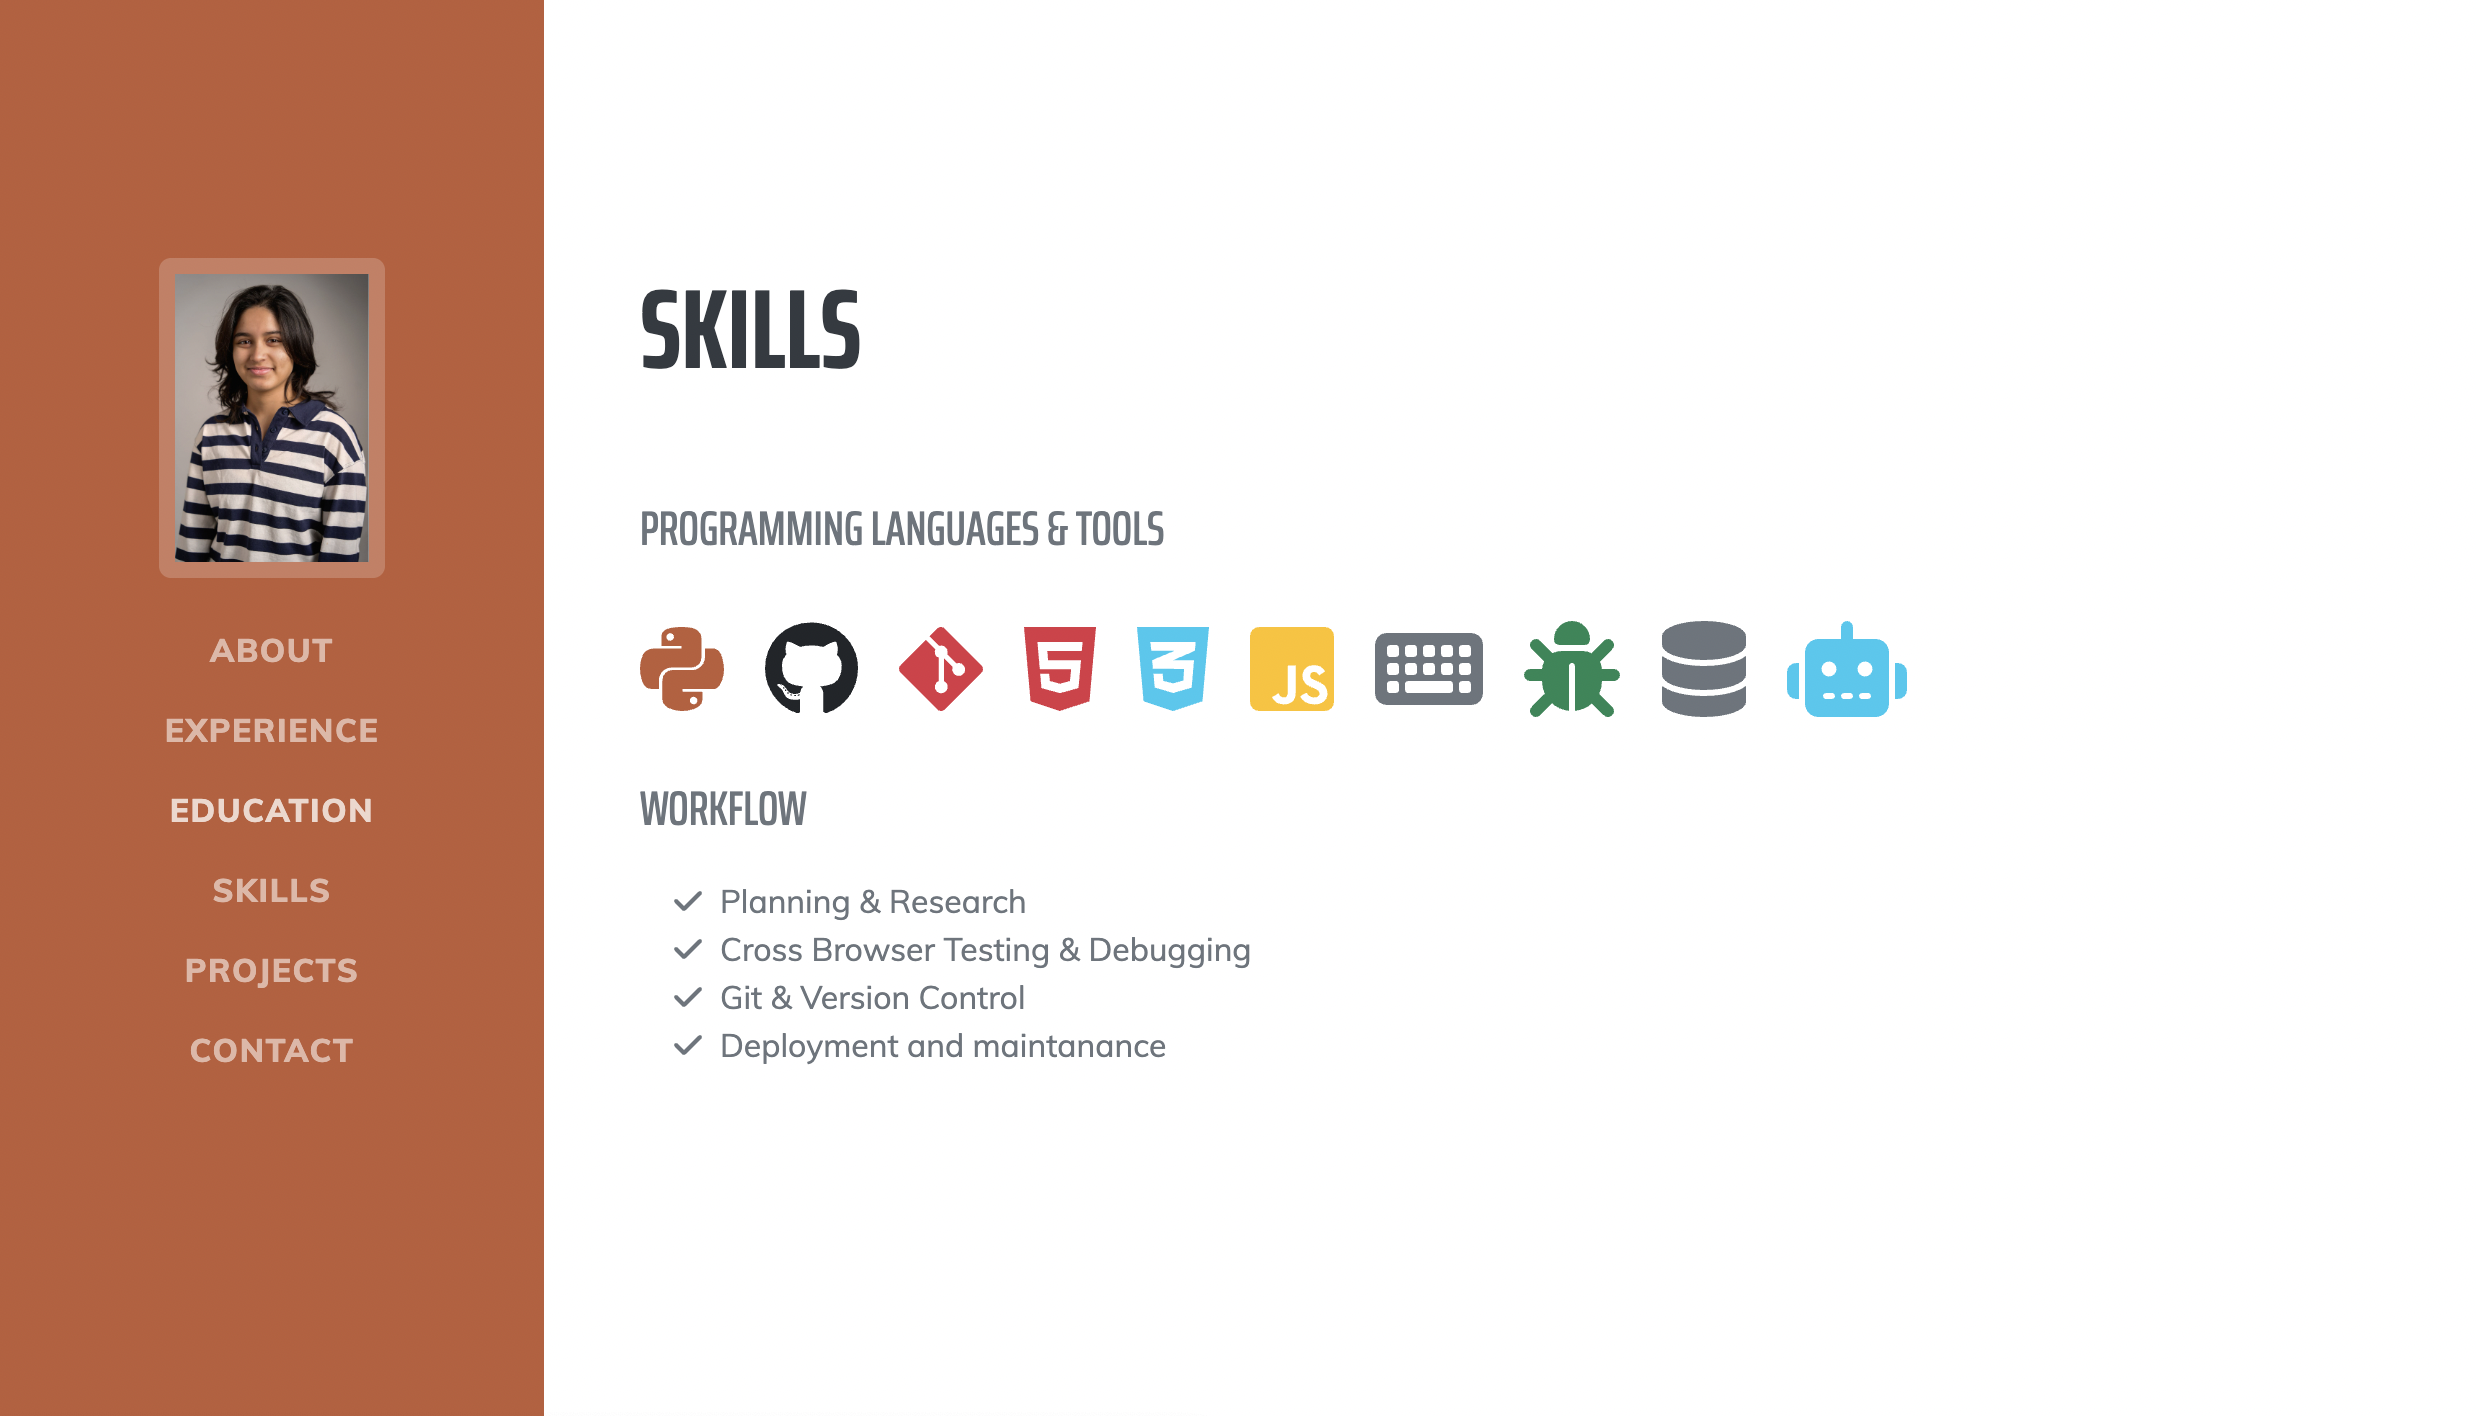
\includegraphics[width=0.75\linewidth]{Screenshot 2026-06-26 at 15.14.10.png}
    \caption{skills}
    \label{skills}
\end{figure}
\newpage
\subsection{Projects}
In this section I have showcase all of my projects.the one I started my coding journey with 
\begin{figure}[h]
    \centering
    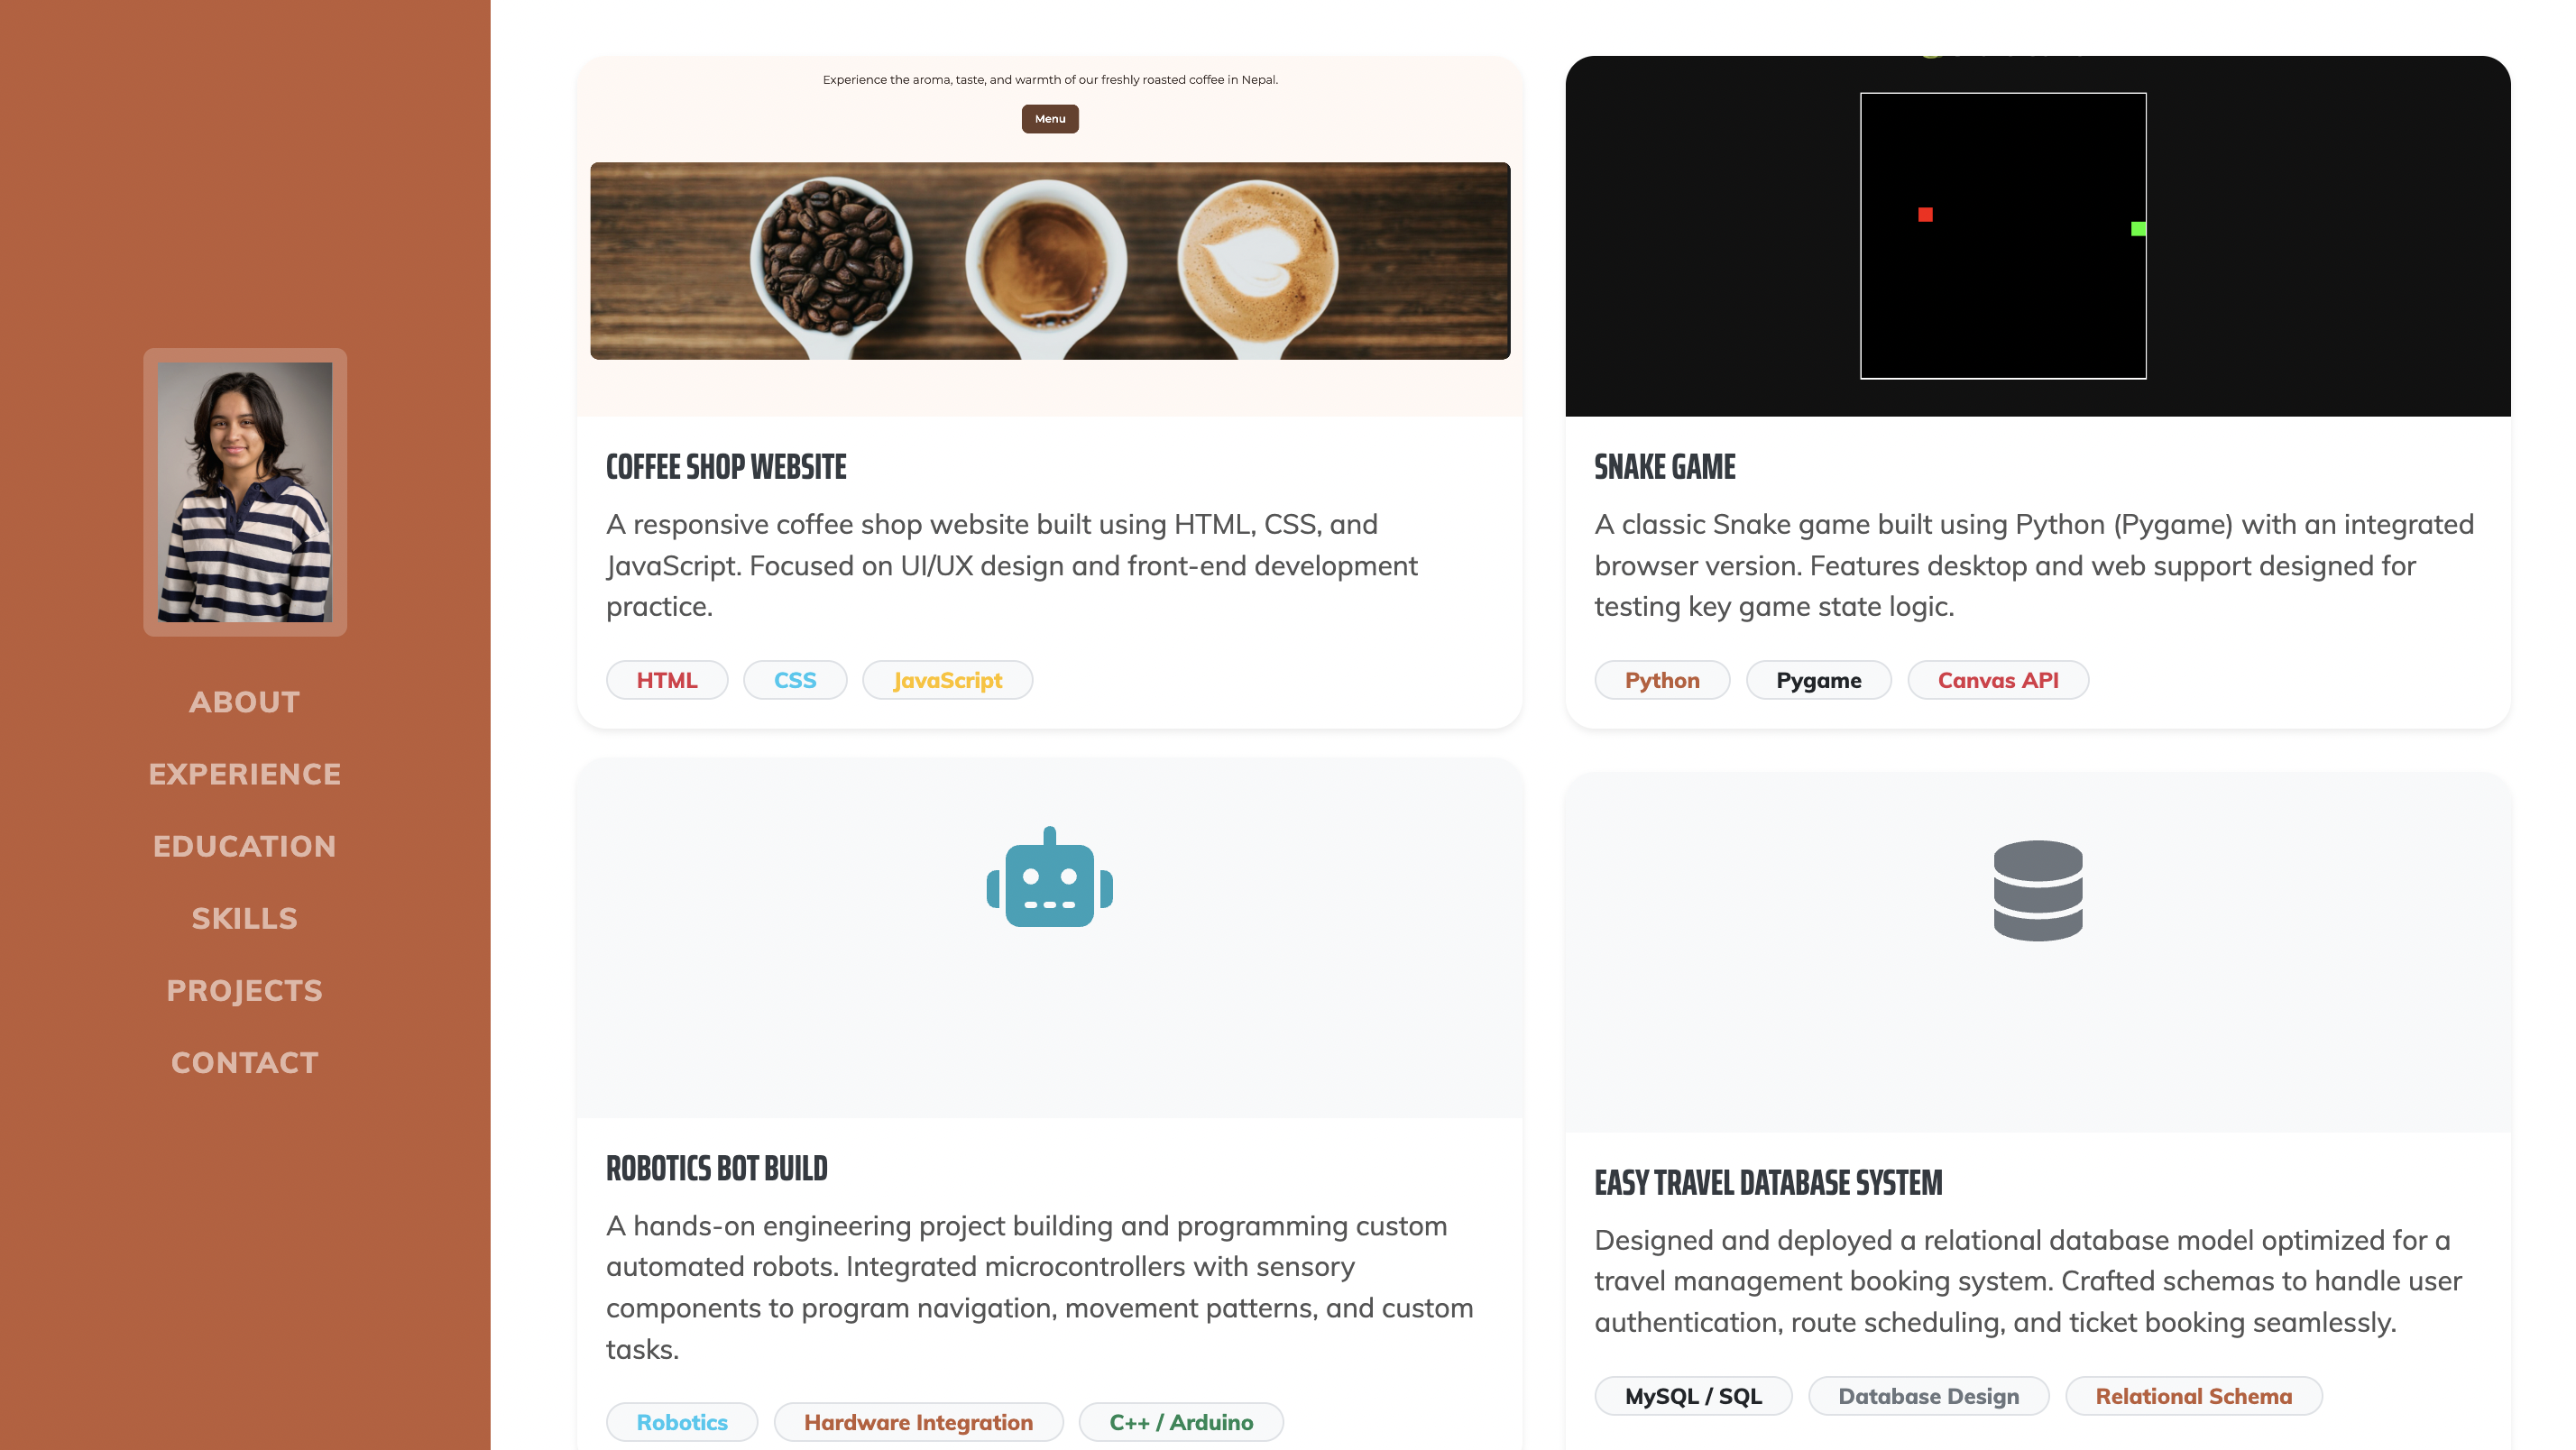
\includegraphics[width=0.57\linewidth]{Screenshot 2026-06-26 at 15.40.43.png}
    \caption{Projects}
    \label{fig:projects}
\end{figure}
\subsection{Contact}
This section was something new for me I used w3wform to create the contact section here you can directly write something to me and it will pop up on my email
\begin{figure}[h]
    \centering
    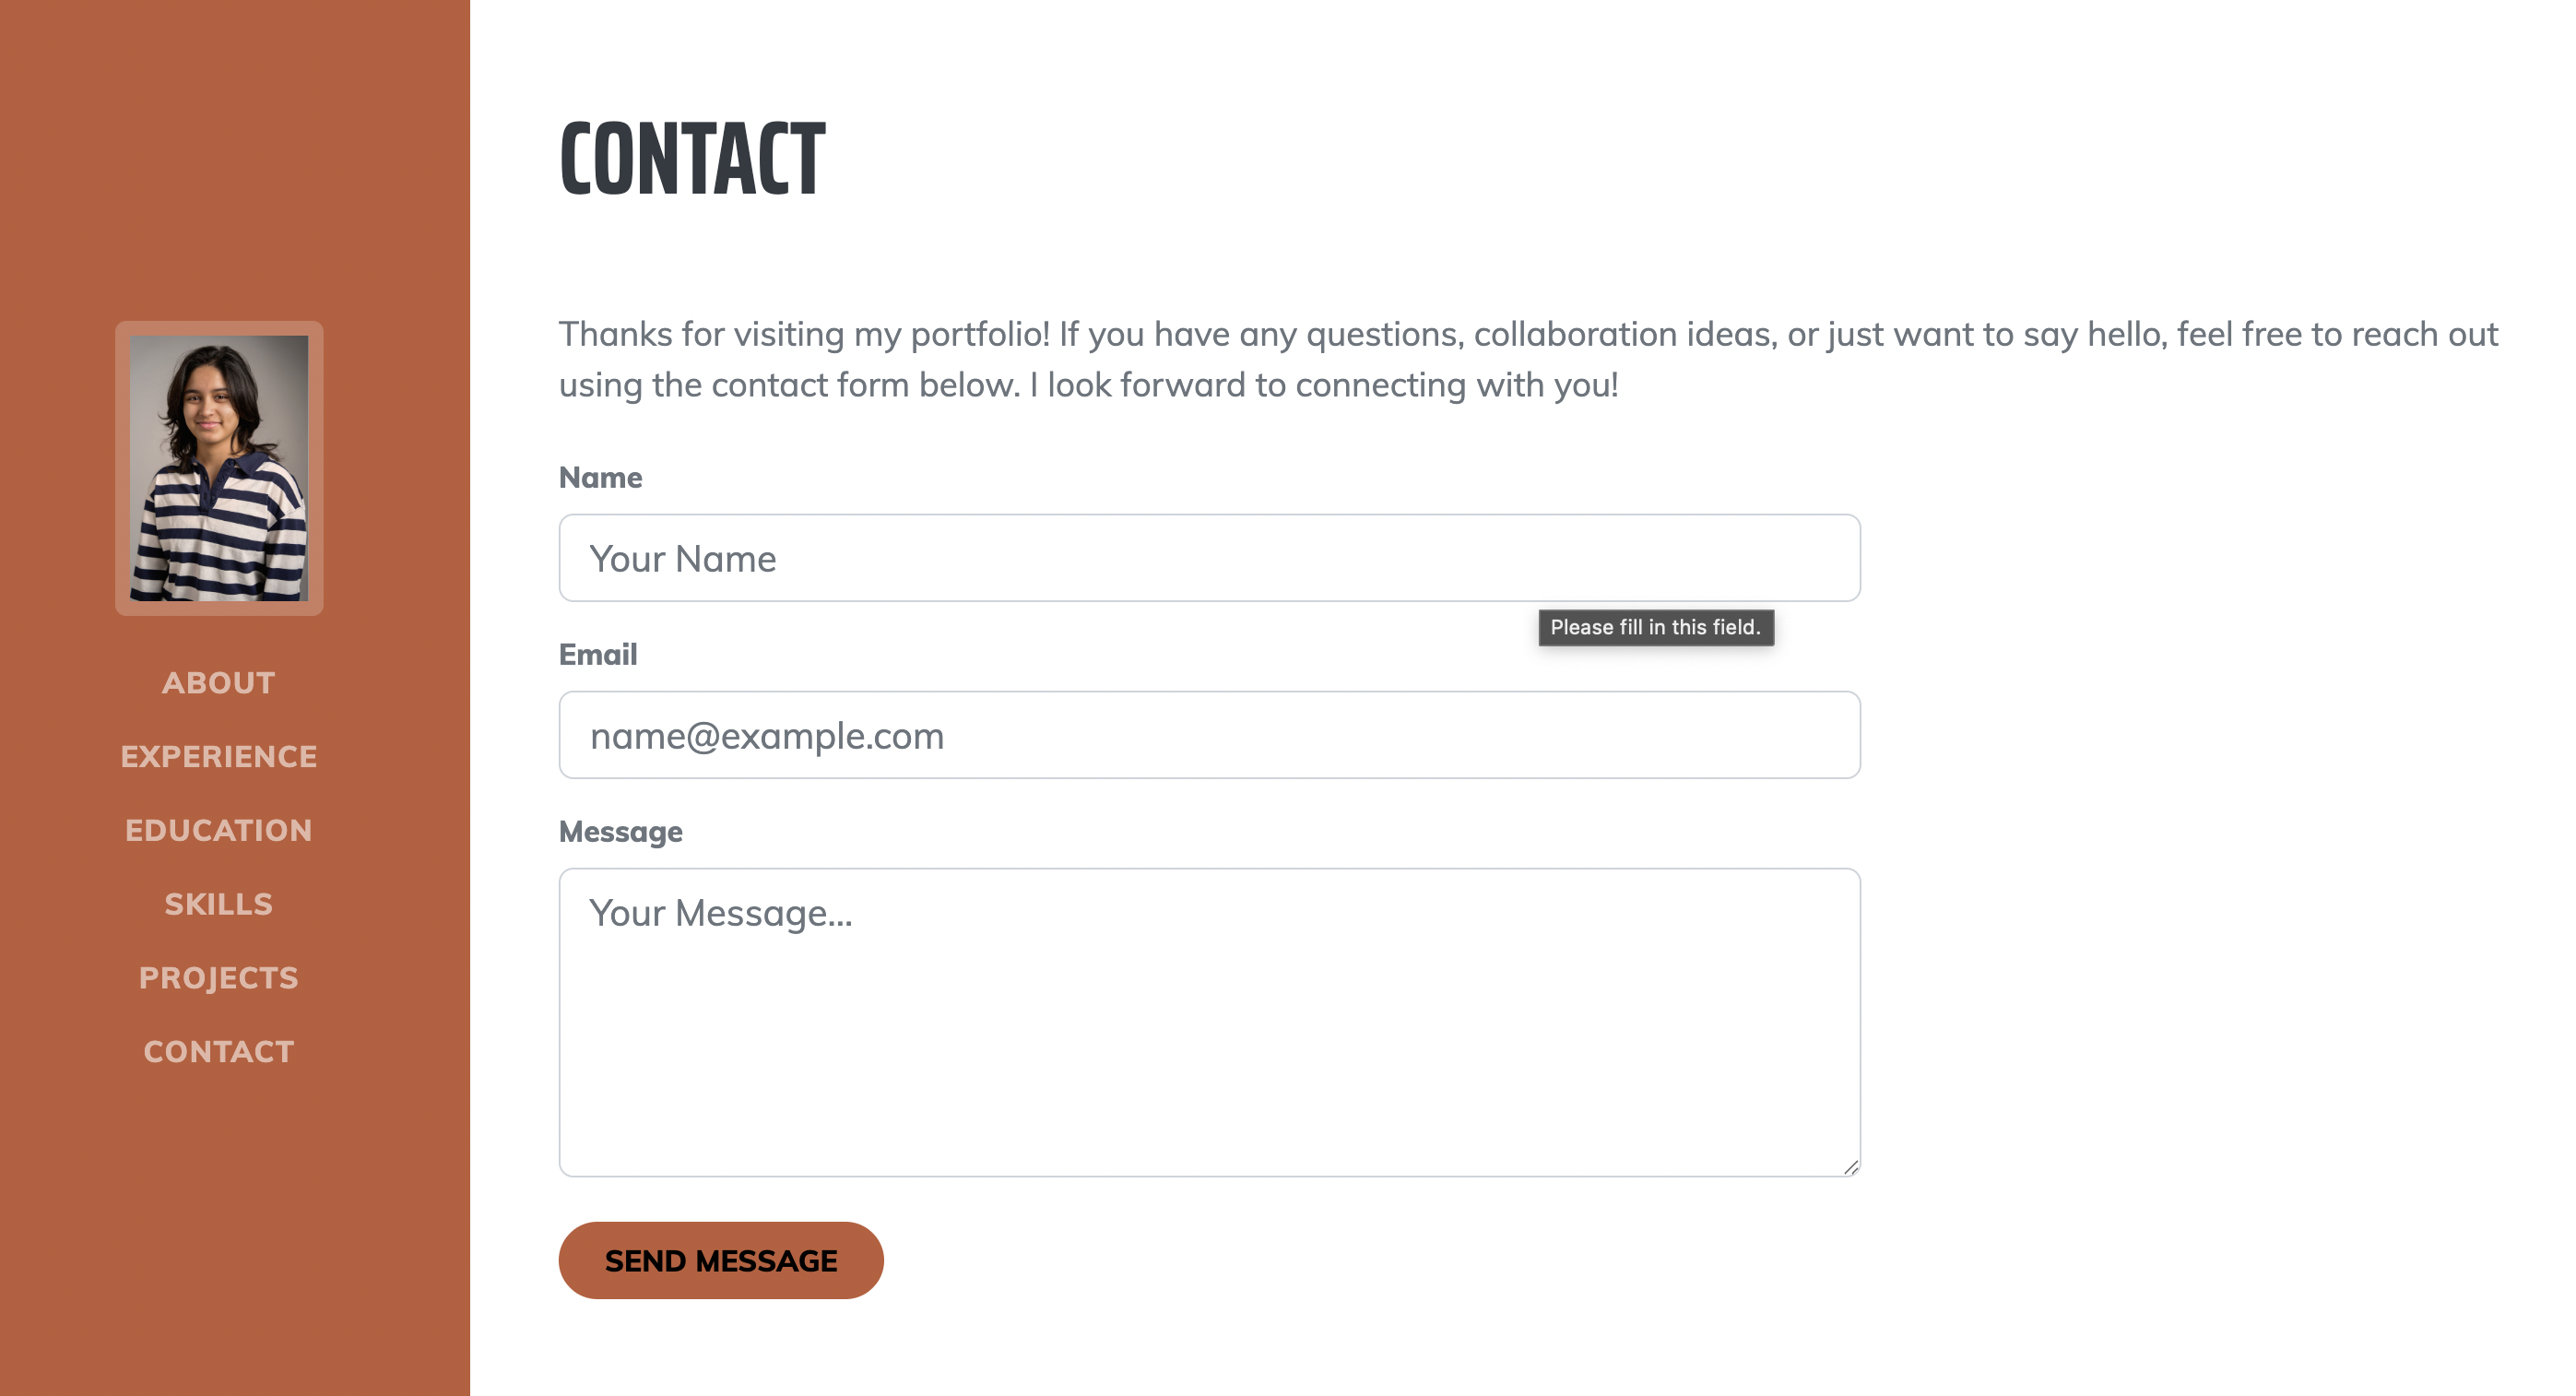
\includegraphics[width=0.75\linewidth]{Screenshot 2026-06-26 at 15.44.20.png}
    \caption{Contact}
    \label{fig: Contact}
\end{figure}
\newpage
\section{Github Repository Structure}
The repository layout separates components clearly to make updates fast and predictable. The structural hierarchy is organized as follows:
\begin{verbatim}

    /Portfolio-computer-lab-
    │
├── index.html          
├── README.md          
├── style.css         
├── script.js         
│
└── /assets
    ├── /images         
    └── subedi_cv.pdf
    
\end{verbatim}

\section{Design decision}
I took serval design decision during this project t o optimize the user journey and maintain a professional layout standards
\begin{itemize}
    \item \textbf{Single page flow:}It's all in one page layout which eliminates the tiring process to go through the pages.Users can smoothly go through my profile in a systematic way simply just by scrolling
    \item \textbf{Color Scheme :} I used orange and white color because it's very bright and catch the direct attention from the user.Black text and times roman font was mostly used in the website to maximize readability and provide strong contrast against the background
    \item \textbf{Contact form:}The website also holds a contact form so that user don't have to go through other socials they can directly email from the website itself
    \item\textbf{Navigation bar:}The navigation bar is always visible beside  the project every time.It was made using CSS and by following css positioning rules
\end{itemize}

\section{Technologies used}
Serval technology were used to develop this portfolio
\begin{itemize}
    \item \textbf{Html5 \& CSS: }Used to develop the foundational layout structure, custom positioning blocks, and typography behaviors.
    \item \textbf{JavaScript (ES):} Manages client-side reactivity and handles layout interactions.
    \item \textbf{W3Forms Integrator:} Added backend processing utility into the web contact section, routing user input strings securely into my mail client inbox.
    \item \textbf{Git \& GitHub Pages:} Used for local repository revision tracking, incremental commit pushes, and live cloud deployment web hosting.
    \item \textbf{LateX:} The specialized processing engine used to cleanly typeset my professional curriculum vitae and this evaluation report.
\end{itemize}
\section{Challenges Encountered During Development}
\subsection{Remote Path Name Sensitivities}
I encountered a lot of issues throught the development process.One of the  challenge involved deploying the website using GitHub Pages.The website was working pretty fine in the local file but while I uploaded it in the github it was a blank page,then after inspecting I found the location of files and images were wrong.

\section{Evaluation and Reflection }
\subsection{Strengths}
My portfolio helps the user to see my skills and my level through it’s easy design and simple navigation. By hosting it to GitHub Page it becomes more reliable and easy to update. Adding the CV made with latex adds more academic touch which will strengthen my professional presentation.

\subsection{Weaknesses}
The contact form entierly relies on external third party like w3wforms for handling user data,instead of deploying an original backend.The descriptions of the project is short as well It would be better if add more details.

\subsection{Future Improvements}
In future I will add some interactive demos like react.I have also decided to integrate active endpoint connection into github's REST API directly.To add a blog to my website where I can write technical articles, tutorials, and share my thoughts.

\subsection{conclusion}
This project report confirms success-full implementation of a personal Software engineering portfolio.The portfolio showcases my educational background, technical skills, and projects while providing an online presence that can be shared with employers and recruiters.




\end{document}
